\documentclass{beamer}
\usepackage[utf8]{inputenc}
\usepackage{gensymb}
\usetheme{Madrid}
\usecolortheme{default}
\usepackage{amsmath,amssymb,amsfonts,amsthm}
\usepackage{mathtools}
\usepackage{txfonts}
\usepackage{tkz-euclide}
\usepackage{listings}
\usepackage{adjustbox}
\usepackage{array}
\usepackage{tabularx}
\usepackage{gvv}
\usepackage{lmodern}
\usepackage{circuitikz}
\usepackage{tikz}
\usepackage{graphicx}

\setbeamertemplate{page number in head/foot}[totalframenumber]

\usepackage{tcolorbox}
\tcbuselibrary{minted,breakable,xparse,skins}



\definecolor{bg}{gray}{0.95}
\DeclareTCBListing{mintedbox}{O{}m!O{}}{%
  breakable=true,
  listing engine=minted,
  listing only,
  minted language=#2,
  minted style=default,
  minted options={%
    linenos,
    gobble=0,
    breaklines=true,
    breakafter=,,
    fontsize=\small,
    numbersep=8pt,
    #1},
  boxsep=0pt,
  left skip=0pt,
  right skip=0pt,
  left=25pt,
  right=0pt,
  top=3pt,
  bottom=3pt,
  arc=5pt,
  leftrule=0pt,
  rightrule=0pt,
  bottomrule=2pt,
  toprule=2pt,
  colback=bg,
  colframe=orange!70,
  enhanced,
  overlay={%
    \begin{tcbclipinterior}
    \fill[orange!20!white] (frame.south west) rectangle ([xshift=20pt]frame.north west);
    \end{tcbclipinterior}},
  #3,
}
\lstset{
    language=C,
    basicstyle=\ttfamily\small,
    keywordstyle=\color{blue},
    stringstyle=\color{orange},
    commentstyle=\color{green!60!black},
    numbers=left,
    numberstyle=\tiny\color{gray},
    breaklines=true,
    showstringspaces=false,
}
%------------------------------------------------------------
%This block of code defines the information to appear in the
%Title page
\title %optional
{3.3.7}

%\subtitle{A short story}

\author % (optional)
{Pratik R-AI25BTECH11023}



\begin{document}


\frame{\titlepage}
\begin{frame}{Question}
A unit vector perpendicular to the plane determined by the points
$P\brak{1,-1,2}$,$Q\brak{2,0,-1}$ and $R\brak{0,2,1}$ is 
\end{frame}
\begin{frame}{Solution}
Let $\myvec{0\\0}$ be the position vector of point $\vec{B}$ and a,b and c be the sides opposite the vertices A,B and C, respectively in $\Delta ABC$.

Given a =8cm;
\begin{align}
    \vec{C}=\myvec{8\\0}
\end{align}
\begin{align}
    \therefore \vec{A}=\myvec{c \cos \angle B\\c \sin \angle B}= \myvec{c\times 1/\sqrt{2}\\c\times 1/\sqrt{2}}
\end{align}
\end{frame}
\begin{frame}{Solution}
in $\Delta ABC$
\begin{align}
   b \cos \angle C + c \cos \angle B = 8
\end{align}
\begin{align}
    b \sin \angle C - c \sin \angle B = 0
\end{align}
Solving linear Equation in b and c:
\begin{align}
    \myvec{\cos \angle C && \cos \angle B \\
    \sin \angle C && -\sin \angle B} \myvec{b \\ c} = \myvec{a\\0}
\end{align}
\end{frame}
\begin{frame}{Solution}
using augmented matrix
\begin{align}
     \myvec{\cos \angle C & \cos \angle B &\vrule &a \\
    \sin \angle C & -\sin \angle B &\vrule &0} 
\end{align}
putting $\angle C = 30\degree$ and $\angle B = 45\degree$
\begin{align}
    \myvec{\sqrt{3}/2 & 1/\sqrt{2} &\vrule &8 \\
    1/2 & -1/\sqrt{2} &\vrule &0}
\end{align}
Echelon form of the matrix is given by 
\begin{align}
    \myvec{\sqrt{3}/2 & 1/\sqrt{2} &\vrule &8 \\
    0 & (-\sqrt{3}-1)/\sqrt{2} &\vrule &-8}
\end{align}
\end{frame}
\begin{frame}{Solution}
\begin{align}
    \frac{(-\sqrt{3}-1)}{\sqrt{2}} \times c = -8
    \end{align}
    \begin{align}
        \implies c = \frac{8\sqrt{2}}{(\sqrt{3}+1)} = \sqrt{3}-1
    \end{align}
    \begin{align}
        \therefore \vec{A}=\myvec{\sqrt{3}-1 \\ 
        \sqrt{3}-1}
    \end{align}
\end{frame}
\begin{frame}{plot}
    \begin{figure}[H]
    \centering
    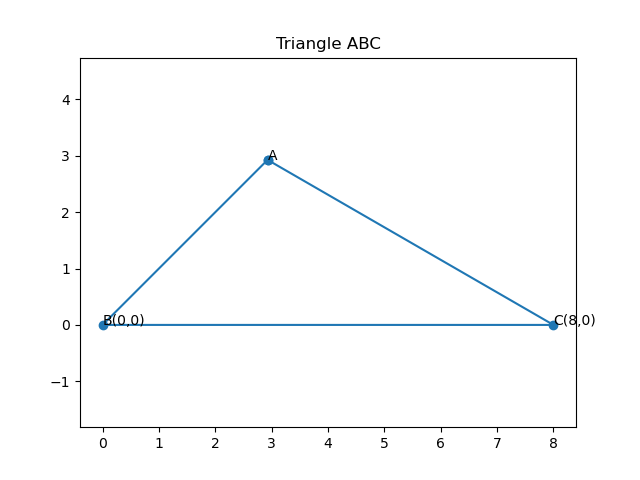
\includegraphics[width=0.6\columnwidth]{../figs/fig.png}   
    \label{fig-1}
\end{figure}
\end{frame}


\end{document}
